\ProvidesFile{seminar06.tex}

\section{Семинар 6}

\subsection{Задача 1}

Докажи, что клетчатый квадрат размера $2^n \times 2^n$
без любой клетки можно разрезать
на уголки, состоящие из трёх клеток.

\begin{proof}
База индукции при $n = 1$ очевидна.

Предположим, что я умею разрезать квадратик $2^n \times 2^n$ без любой клетки на уголки, состоящие из трёх клеток, и мне дали любой квадрат $2^{n+1} \times 2^{n+1}$ без любой клетки.

Первое, что нужно сделать -- разрезать его на 4 квадрата $2^n \times 2^n$ как показано на рисунке:

\begin{figure}[H]
    \centering
    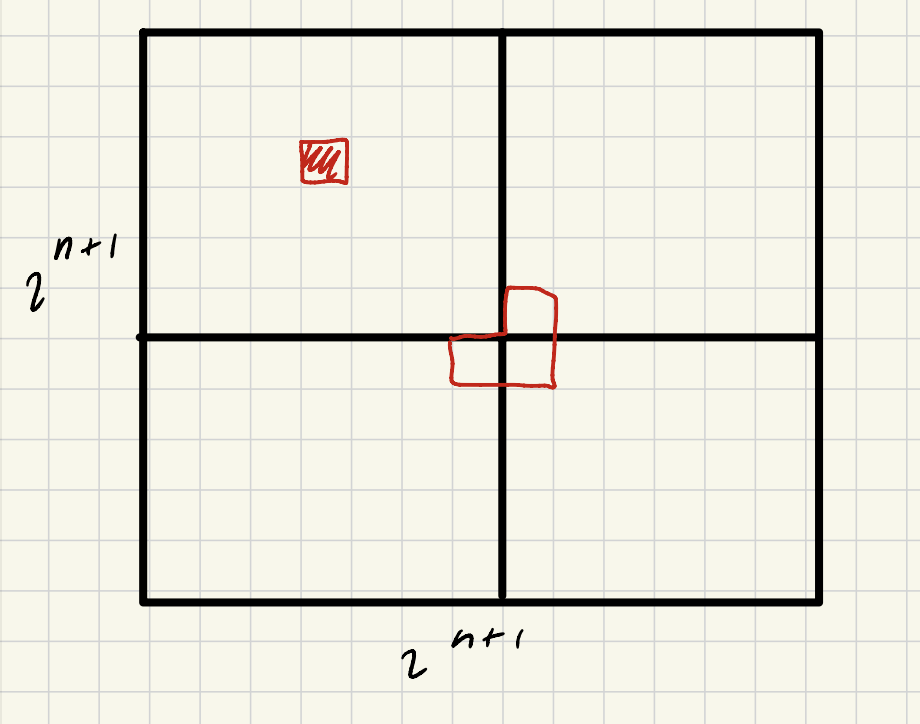
\includegraphics[width=0.5\linewidth]{Figures/sem06_task1.png}
    \caption{Заштрихованная красная клетка отсутствует в квадрате $2^{n+1} \times 2^{n+1}$}
    \label{fig:enter-label}
\end{figure}

Тогда отсутствующая клетка попадает в один из этих квадратов. Но тогда в оставшихся трёх я могу вырезать по клетке так, чтобы в итоге образовался уголок (аналогично картинке). Тогда получается 4 квадрата $2^n \times 2^n$. По предположению индукции я умею разрезать квадрат $2^n \times 2^n$ без любой клетки на уголки, состоящие из трёх клеток. Поэтому я смогу разрезать каждый из четырех квадратов на уголки. Значит, и весь квадрат $2^{n+1} \times 2^{n+1}$ без одной клетки тоже побьётся на уголки. Переход доказан.
\end{proof}

\subsection{Задача 2}

На плоскости провели $n$ прямых так, что любые две проведённые прямые пересекаются, и никакие три прямые не пересекаются в одной точке. На сколько частей прямые поделят плоскость?

Посмотрим, как устроен ответ при маленьких $n$:

\begin{table}[h]
\centering
\begin{tabular}{|c|c|}
\hline
\textbf{Кол-во прямых} & \textbf{Кол-во частей плоскости} \\ \hline
0 & 1 \\ \hline
1 & 2 \\ \hline
2 & 4 \\ \hline
3 & 7 \\ \hline
4 & 11 \\ \hline
\end{tabular}
\end{table}

Возникает гипотеза, что ответ вычисляется по такой формуле:
\[
\frac{n(n + 1)}{2} + 1
\]
\begin{proof}
Докажем это по индукции:

\textbf{База индукции.} при $n = 0$ очевидна.

\textbf{Предположение индукции.} Предположим, что $n$ прямых делят плоскость на $\frac{n(n+1)}{2} + 1$ частей

\textbf{Доказательство перехода индукции.} Хотим доказать, что $n + 1$ прямая делит плоскость на $\frac{(n+1)(n+2)}{2} + 1$ частей.

Давайте выкинем из конструкции с $n + 1$ прямой одну прямую, проверим, что она является корректной конструкцией (любые две проведённые прямые пересекаются, и никакие три прямые не пересекаются в одной точке, далее такие конструкции называются конструкцией общего положения) из условия с $n$ прямыми, а затем убедимся в верности утверждения для $n + 1$.

\textbf{Важно:} мы делаем именно так, а не прибавляем к $n$ прямых ещё одну потому что не ясно, почему это не испортит конструкцию из условия.

Действительно: если мы из конструкции с $n + 1$ прямых общего положения выкидываем одну прямую, то получаем конструкцию общего положения из $n$ прямых. Следовательно, в ней есть ровно $\frac{n(n+1)}{2} + 1$

Давайте вернем выкинутую прямую и проверим, что с ней тоже утверждение.

По условию любые 2 прямые пересекаются, следовательно, $n+1$ прямая пересекается с $n$ прямыми. Они разбивают эту прямую на $n + 1$ кусок. При этом каждый кусок лежит ровно в одной <<старой>> части плоскости. 

\begin{figure}[H]
    \centering
    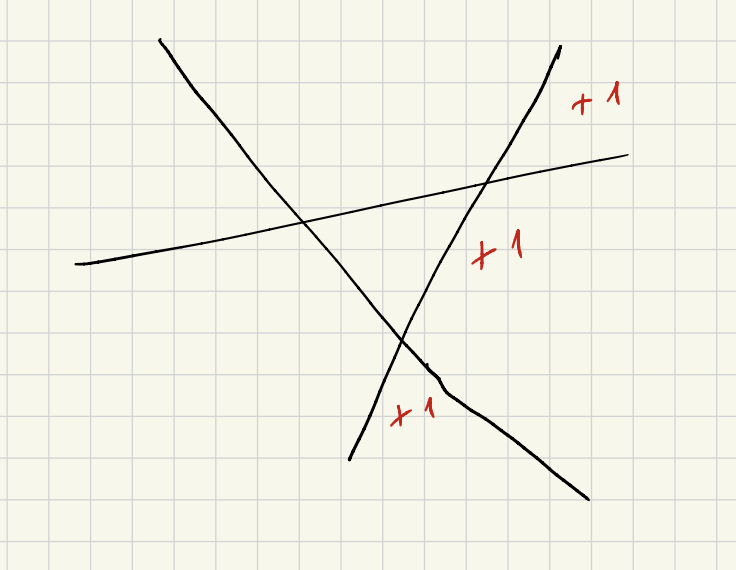
\includegraphics[width=0.5\linewidth]{Figures/sem06_task2.png}
\end{figure}

Тогда ясно, что каждый кусок прямой разбивает свою часть плоскости на две. То есть, делает вклад +1 к количеству частей. Значит, всего добавится $n + 1$ часть.
\[
\frac{n(n+1)}{2} + 1 + n + 1 = \frac{(n+1)(n+2)}{2} + 1
\] 
Переход индукции доказан.
\end{proof}

\subsection{Задача 3}

Шеренга новобранцев стоит перед старшиной. Он командует «налево». По неопытности часть солдат поворачивается налево, а часть – направо. После этого каждую
секунду происходит следующее: солдаты, оказавшиеся друг к другу лицом, понимают, что произошла ошибка, и поворачиваются кругом. В следующую секунду ситуация
повторяется. Докажи, что рано или поздно шеренга встанет неподвижно.
Эту задачу можно было бы решить с помощью полуинвариантов. Но сейчас мы предлагаем
решить ее индукцией по числу солдат.

\begin{proof}
Будем доказывать индукцией по $n$ (числу солдат).

База индукции при $n = 1$ очевидна.

Рассмотрим $n + 1$ солдата. Если к нему никто никогда не поворачивается лицом, то забываем про этого солдата и рассматриваем оставшихся $n$.

Если же к нему кто-нибудь когда-нибудь повернется лицом, то он отвернется от этого человека и будет смотреть в воздух, и уже больше точно никогда не повернется и опять перейдем к оставшимся $n$ солдатам.
\end{proof}

\subsection{Задача 4}

Скорее всего, в задаче опечатка, иначе она из милой доброй задачи про рекурру превращается в жуткий гроб с бесконечным счётом. Буду решать в такой формулировке:

Реши рекуррентное уравнение:
\[
x_0 = 43, x_1 =70, \quad x_{n+2} = 29x_{n+1} - 28x_{n}
\]
Решаем характеристическое уравнение.
\[
\lambda^2 - 29\lambda + 28 = 0
\]
Корни:
\[
\lambda_1 = 28, \quad \lambda_2 = 1
\]
Общее решение:
\[
x_n = A \cdot 28^n + B
\]
Найдем константы:
\[
\begin{cases}
    A + B = 43, \\
    28A + B = 70
\end{cases} \implies A = 1, \quad B = 42
\]
Итоговое решение:
\[
x_n = 28^n + 42
\]

\textbf{Ответ:} $x_n = A \cdot 28^n + B$

\subsection{Задача 5}

Зайчик стоит у подножия лесенки высотой n ступенек. За один прыжок он может подняться либо на одну, либо на две ступеньки вверх. Сколькими способами он может
добраться до верха?

Пусть $x_k$ -- число способов прыгнуть в $k$-ую ступеньку. Ясно, что $x_k = x_{k-1} + x_{k-2}$, так как зайчик может прыгнуть в $k$-ую ступеньку либо с $k-1$ ступеньки, либо с $k - 2$ ступеньки.

Тогда это просто задача про рекуррентное уравнение вида 
\[
x_k = x_{k-1} + x_{k-2}
\]

Ясно, что на первую ступеньку зайчик может прыгнуть только с самого низа (1 способ), а на вторую -- либо с самого низа, либо с первой ступеньки (2 способа).

Тогда $x_n = F_{n+2}$, где $F_{i}$ - $i$-ое число Фибоначчи.

\textbf{Ответ:} $x_n = F_{n-2}$

\subsection{Задача 6}

Есть 2 принципиально разных способа получить прямоугольник $2 \times n$.

\begin{figure}[H]
    \centering
    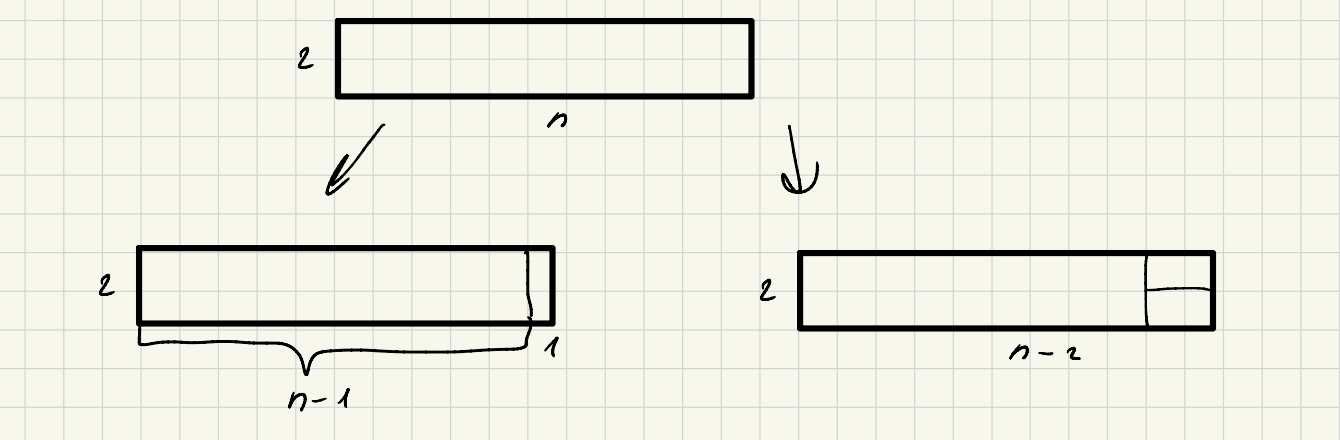
\includegraphics[width=1\linewidth]{Figures/sem06_task6.png}
\end{figure}

Либо из прямоугольника $2 \times (n-1)$ прибавлением одной доминошки, либо из прямоугольника $2 \times (n -2)$ прибавлением двух доминошек.

Получаем рекуррентное уравнение $x_n = x_{n-1} + x_{n-2}$, где $x_i$ -- число способов получить прямоугольник $2 \times i$

Тогда ясно, что ответ на задачу -- это числа Фибоначчи (возможно, с каким-то сдвигом).

$x_1 = 1$ (одна вертикальная доминошка)

$x_2 = 2$ (две вертикальных, либо две горизонтальных доминошек).

Тогда ясно, что $x_i = F_{i+2}$

\textbf{Ответ:} $F_{i+2}$

\subsection{Задача 7}

Докажи тождества для всех натуральных $m, n$:

\begin{enumerate}[label=\asbuk*)]
\item \textbf{(тождество Кассини)} $F_{n+1} \cdot F_{n-1} - F_n^2 = (-1)^n$
\item $F_{m+n} = F_m \cdot F_{n+1} + F_{m-1} \cdot F_{n}$
\item $F_{2n+1} = F^2_n + F^2_{n+1}$
\end{enumerate}

\subsubsection{Пункт Б}
\[
F_{m+n} = F_m \cdot F_{n+1} + F_{m-1} \cdot F_{n}
\]
\begin{proof}
Проверим базу при $n = 1$:
\[
F_{m+1} = F_{m} \cdot F_{2} + F_{m-1} F_{2} = F_m + F_{m-1}
\] 

Верность равенства очевидна в силу определения чисел Фибоначчи. Заметьте, что это равенство верно при любом $m$ (ну то есть я никак не пользуюсь тем, чему равно $m$).

Предположим, что $F_{m+n} = F_m \cdot F_{n+1} + F_{m-1} \cdot F_{n}$ при всех значениях $\leq n$.

Докажем, что тогда формула верна и для $n + 1$, то есть покажем справедливость формулы:
\[
F_{m+n+1} = F_m \cdot F_{n+2} + F_{m-1} \cdot F_{n+1}
\]

По определению чисел Фибоначчи:
\[
F_{m+(n+1)} = F_{m+n} + F_{m+(n-1)}
\]
Воспользуемся предположением индукции:
\[
F_{m+(n+1)} = F_{m} \cdot F_{n+1} + F_{m-1} \cdot F_n + F_m \cdot F_n + F_{m-1} \cdot F_{n - 1} = F_m(F_{n+1} + F_{n}) + F_{m - 1} \cdot (F_n + F_{n-1}) = F_m \cdot F_{n+2} + F_{m-1} \cdot F_{n+1}
\]

Это доказывает переход по $n$. А для $m$ не надо доказывать, так как мы нигде его не фиксировали.
\end{proof}

\subsubsection{Пункт В}
\[
F_{2n+1} = F^2_n + F^2_{n+1}
\]
\begin{proof}
Воспользуемся результатом из пункта Б для $m := n + 1, n := n$ ($F_{m+n} = F_m \cdot F_{n+1} + F_{m-1} \cdot F_{n}$)
Получим:
\[
F_{n +(n+1)} = F_{n+1} \cdot F_{n+1} + F_{n} \cdot F_{n} = F^2_n + F^2_{n+1}
\]
\end{proof}

\subsection{Задача 8}

Ясно, что из условия возникает следующее рекуррентное уравнение:
\[
x_n = x_{n-1} + 6x_{n-2}
\]

Решаем характеристическое уравнение:

$\lambda^2 - \lambda - 6 = 0$

$\lambda_1 = -2, \lambda_2 = 3$

Тогда: 
\begin{equation}
    x_n = c_1 \cdot (-2)^n + c_2 \cdot 3^n
    \label{equation::reucur}
\end{equation}

У нас есть два условия: $x_0 = 0, x_1 = 1$.

Подставим $n = 0$ и $n = 1$ в уравнение \ref{equation::reucur} и получим:

\begin{equation*}
\begin{cases}
    0 = c_1 + c_2 \\
    1 = -2c_1 + 3c_2
\end{cases}
\end{equation*}

Решая эту систему находим: $c_1 = -1/5, c_2 = 1/5$

\textbf{Ответ:} $x_n = \frac{1}{5}(3^n - (-2)^n )$
\subsection{Задача 9}

Пусть: $A_n$ -- количество способов добраться от $A$ до $A$ за $n$ шагов. \\
$B_n$ -- количество способов добраться от $A$ до $B$ за $n$ шагов. \\
$C_n$ -- количество способов добраться от $A$ до $C$ за $n$ шагов. \\
$D_n$ -- количество способов добраться от $A$ до $D$ за $n$ шагов.

Заметим, что $A_n$ = $C_n$. Действительно: в эти вершины я могу прийти только из $B$ или $D$. 

Аналогично: $B_n = D_n$

Так как в $A$ можно попасть либо из $B$, либо из $D$, то: $A_n = 2B_{n-1}$

Аналогично: $B_n = 2A_{n-1}$. Подставим это в уравнение строчкой выше:

\begin{equation}
   A_n = 4A_{n-2}
   \label{equation::recur2}
\end{equation}

Ясно, что: $A_1 = 0$, $A_2 = 2$

Тогда решая рекуррентное уравнение \ref{equation::recur2}, получаем:
$A_{2k+1} = 0$

$A_{2k} = 2^{2k-1}$

\textbf{Ответ:} если $n = 2k + 1$, то 0. если $n = 2k$, то $2^{2k-1}$

\subsection{Задача 10}

Приложу картинку, из которой примерно можно понять идею решения, нет времени подробно расписывать.

\begin{figure}[H]
    \centering
    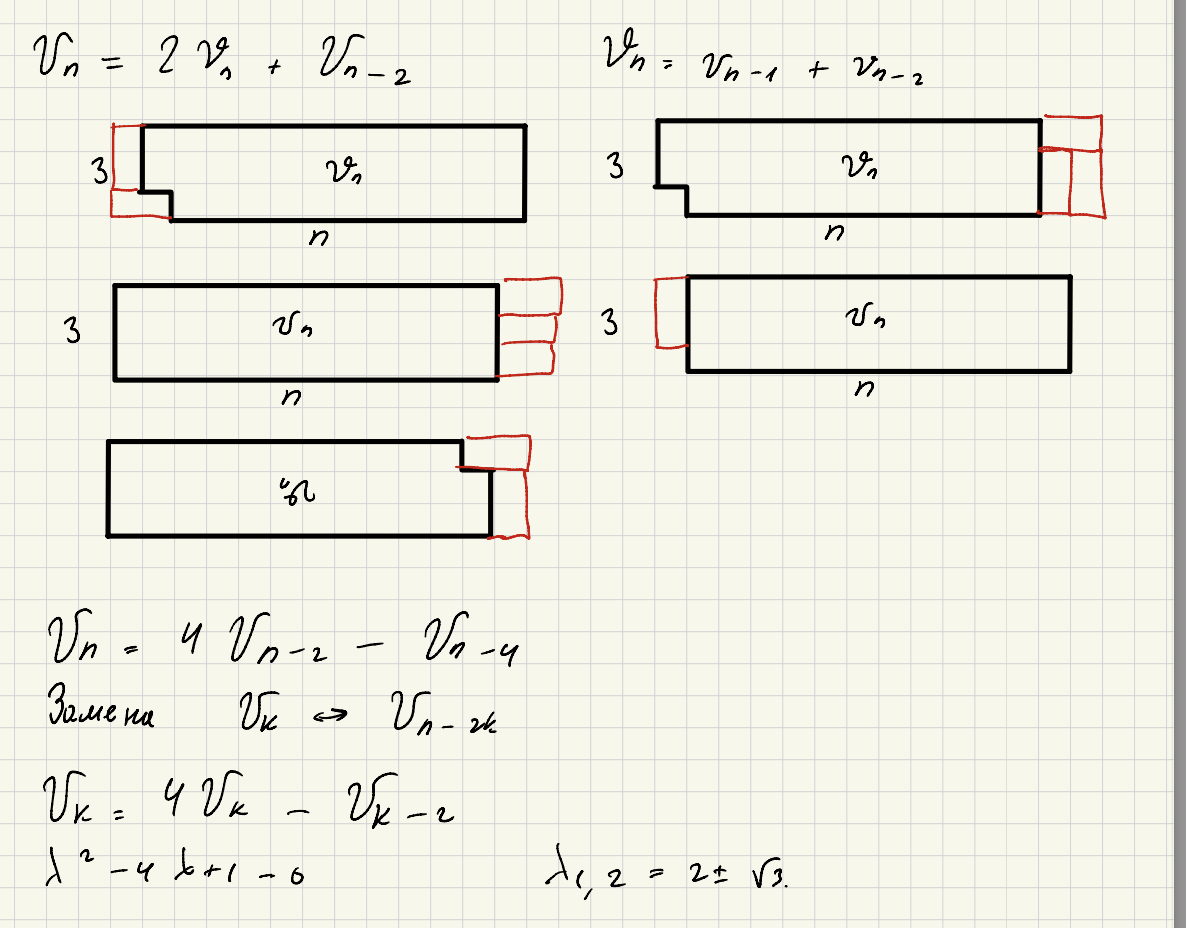
\includegraphics[width=0.75\linewidth]{Figures/sem06_task10.png}
\end{figure}